\documentclass[a4paper,12pt]{report} 
\usepackage[utf8x]{inputenc}
\usepackage[french]{babel}
\usepackage{mathtools}
\usepackage{amsmath, amssymb, amsfonts}
\usepackage{textcomp}
\usepackage[nointegrals]{wasysym}			% Collection de symboles mathématiques
\usepackage{ifthen}
\usepackage{tabularx}	 				% Gestion avancée des tableaux
%\usepackage{cleveref}

\usepackage{enumitem}
\usepackage{wrapfig}
%\usepackage[squaren]{SIunits}
%\usepackage[T1]{fontenc}				% Indispendable, présent dans tous les codes exemples
\usepackage[linkcolor=Indigo,colorlinks=true, citecolor=SaddleBrown, urlcolor=MidnightBlue]{hyperref} 	% Hyper ref
\usepackage{listings}					% Pour citer du code
\usepackage[justification=centering]{caption}
\usepackage{sistyle} 
\usepackage{numprint}
\usepackage{wrapfig}
\usepackage{cite}	
\usepackage{url} 					% Pour citer les sites internet dans la
%\usepackage{cleveref}
\usepackage{setspace}

\usepackage{graphicx}		 			% Inclusion des figures
\graphicspath{{./pic/}}
\usepackage[svgnames]{xcolor}			%https://www.latextemplates.com/svgnames-colors

%%% Commandes utiles définies
\newcommand{\argmin}{\mathop{\mathrm{argmin}}}

\newcommand{\bepar}[1]{
	\left( #1 \right)  
}

\newcommand{\becro}[1]{
	\left[ #1 \right]  
}

\newcommand{\beacc}[1]{
	\left\{ #1 \right \}  
}

\newcommand{\norm}[1]{
	\left \vert \left \vert #1 \right \vert  \right \vert
}

\newcommand{\rbk}[1]{\color{red}\textit{#1} \color{black}  
}

\usepackage{listings}					% Pour citer du code
%%%%%%%%%%%%%%%%%%%
%%% Élément pour citer des codes %%%
\lstset{
language=Python,
basicstyle=\ttfamily\bfseries\small, %
identifierstyle=\bfseries\color{black}, %
keywordstyle=\color{blue}, %
stringstyle=\color{black!90}, %
commentstyle=\it\color{black!70}, %
columns=flexible, %
tabsize=4, %
extendedchars=true, %
showspaces=false, %
showstringspaces=false, % %
numberstyle=\small, %
breaklines=true, %
breakautoindent=true, %
captionpos=b,
otherkeywords={cross_val_score},
keywords=[0]{cv},
keywordstyle=[0]{\color{red}},
}
%%%%%%%%%%%%%%%%%%%%%
\title{\navy \textbf{Notes bibliographiques : \\ Utilisation de ML pour la turbulence} \color{black}}%%%%%%%%%%%%%%%%%%%%
\date{}
%\usepackage{multicol}
%\usepackage{etoolbox}
%\patchcmd{\thebibliography}{\section*{\refname}}
%    {\begin{multicols}{2}[\section*{\refname}]}{}{}
%\patchcmd{\endthebibliography}{\endlist}{\endlist\end{multicols}}{}{}
\usepackage[authoryear]{natbib}

\usepackage{geometry}
\geometry{hmargin=2cm, vmargin=2cm}

%%%%%%%%%%%%%%%%%%%%
%%% Couleurs %%%
\xdefinecolor{brick}{named}{DarkRed}
\xdefinecolor{navy}{named}{Navy}
\xdefinecolor{midblue}{named}{MidnightBlue}
\xdefinecolor{dsb}{named}{DarkSlateGray}
\xdefinecolor{dgreen}{named}{DarkGreen}
\xdefinecolor{indian}{named}{IndianRed}

%%% 	Raccourcis 	%%%
\newcommand{\keps}{$k-\varepsilon$}
\newcommand\bk{\color{black}}
\newcommand\brick{\color{brick}}
\newcommand\navy{\color{navy}}
\newcommand\midblue{\color{midblue}}
\newcommand\dsb{\color{dsb}}
\newcommand{\dgreen}{\color{dgreen}}
\newcommand{\dpurple}{\color{indian}}
\newcommand\red{\color{red}}

%%%%%%%% Cigles
\newcommand{\rap}{par rapport}
\newcommand{\cad}{c'est-à-dire}
\newcommand{\vav}{vis-à-vis}

%%%%%%%% Autres

%%%%%%%%%%%%%%%%%%%
% Syntax: \colorboxed[<color model>]{<color specification>}{<math formula>}
\newcommand*{\colorboxed}{}
\def\colorboxed#1#{%
  \colorboxedAux{#1}%
}
\newcommand*{\colorboxedAux}[3]{%
  % #1: optional argument for color model
  % #2: color specification
  % #3: formula
  \begingroup
    \colorlet{cb@saved}{.}%
    \color#1{#2}%
    \boxed{%
      \color{cb@saved}%
      #3%
    }%
  \endgroup
}
\renewcommand{\sectionmark}[1]{\markright{#1}}
\usepackage{fancyhdr}
\pagestyle{fancy}
\lhead{\textbf{Nathaniel} \brick \textbf{\textsc{Saura}}}
\rhead{\markright}
\cfoot{\thepage}
\renewcommand{\headrulewidth}{0.4pt}

\numberwithin{equation}{section} %%%% To count the equation like Section.Number

\usepackage{accents}
\newcommand{\vect}[1]{\accentset{\Rightarrow}{#1}}

\usepackage{multicol}		% Pour utiliser \hfill et découper une partie de son texte en colonnes
\setlength{\columnseprule}{0.1pt}
\def\columnseprulecolor{\color{red}}
\setlength{\columnsep}{1.5cm}

% Numéro Roman pour le texte
\makeatletter
\newcommand*{\rom}[1]{\expandafter\@slowromancap\romannumeral #1@}
\makeatother

\begin{document}
\maketitle
\newcolumntype{M}[1]{>{\centering\arraybackslash}m{#1}}
\newcolumntype{N}{@{}m{0pt}@{}}

%\noindent On se base sur \textbf{\citep{ling2016machine}} qui se pose la question de comment inculquer les propriétés d'invariance lors de l'apprentissage, et de voir si le faire améliore les prédictions.
\subsection*{\textbf{\cite{singh2017machine}} : }
\noindent L'idée de cet article peut être schématisée par la figure suivante (extraite de l'article) :

\begin{figure}[!ht]
\centering
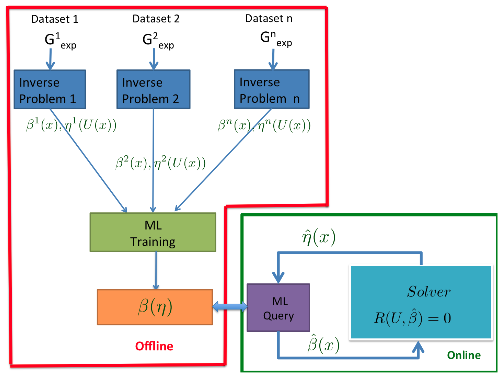
\includegraphics[scale=0.8 ]{singh.png}
\caption{Schéma des trois étapes pour augmenter les modèles de la turbulence}
\label{singh}
\end{figure}

\noindent Le modèle SA peut être représenté par 
\begin{equation}
\frac{D \tilde{\nu}}{Dt} = P\bepar{\tilde{\nu}, \textbf{U}} - D\bepar{\tilde{\nu}, \textbf{U}} + T\bepar{\tilde{\nu}, \textbf{U}}
\end{equation}
La grandeur $\tilde{\nu}$  est liée avec la viscosité turbulente $\nu_t$ de Boussinesq (Voir annexe 3 de l'article).\\
L'idée de l'article et des méthodes développées par \cite{parish2016paradigm} est d'inférer un terme de correction. En effet, les modèles (SA, $k-\varepsilon$) simplifient certains termes de Navier-Stokes (DNS). Du coup, en rajoutant un terme dynamiquement adaptable au cours du processus d'inférence Baysienne, on serait à priori capable de retrouver la véritable physique.\\
Le grand défi réside dans la généralisation de cette correction, et c'est là où l'injection d'une prédiction via les MLA(lgorithmes) devient inévitable.\\
Ce terme est injecté dans le terme de production. Le modèle s'écrit alors :
\begin{equation}
\frac{D \tilde{\nu}}{Dt} = \beta\bepar{\textbf{x}}P\bepar{\tilde{\nu}, \textbf{U}} - D\bepar{\tilde{\nu}, \textbf{U}} + T\bepar{\tilde{\nu}, \textbf{U}}
\end{equation}
Leur inversion peut sembler différente de celle effectuer dans \cite{parish2016paradigm} ou \cite{tarantola2005inverse} mais finalement la régression de Tikhonov (L1 et L2) avec un facteur de régression $\lambda = 4 \times 10^{-4}$ (similaire dans le sens au learning rate dans le NN) peut être ramener à ce qui est décrit dans les articles précédemment cités. \\
Dans notre article, l'inférence se fait sur le coefficient de portance $C_l$, la fonction de coût s'écrit alors :
\begin{equation*}
\mathcal{J} = \underset{\beta}{\text{min}}\becro{\sum^{N_d}_{j=1}\becro{C_{l,\text{exp}} - C_l\bepar{\beta}}^2  + \lambda \sum^{N_m}_{n=1} \becro{\beta\bepar{x_n}-1}^2}
\end{equation*}

\noindent On peut expliquer les termes de cette équation : 
\begin{itemize}[leftmargin=10mm]
\item[-- ] $N_d$ : le nombre de points où sont réalisées les mesures expérimentales. Le coefficient de portance étant un champ, ces valeurs scalaires dépendent dre la position sur l'aile (par exemple)
\item[-- ] $N_m$ : le nombre de volumes de contrôle, \cad $ $ le nombre de points de \textit{maillage} sur l'aile mais également autour, puisque dans ce genre de cas le contexte à son importance.
\item[-- ] $\lambda$ : ampleur de la régression L1. Par rapport à l'article \cite{parish2016paradigm} $\lambda$ peut être vu comme le rapport des covariances observées sur \textit{prior} : $$ \lambda = \frac{C_\text{pri}^{-1}}{C_\text{obs}^{-1}} = \frac{C_\text{obs}}{C_\text{pri}} $$ Sachant cela, les carrés représentent alors le produit scalaire et on peut faire un analogie avec l'expression de la fonction de coût \cite{parish2016paradigm}.\\
D'un point de vue plus algorithmique, augmenter $\lambda$ revient à augmenter la \textit{sparsity} des données inférées \textit{i.e} ne pas temnir compte des actions faibles de certains éléments.
\end{itemize}

\noindent Il est également mentionné qu'en utilisant le coefficient de pression de surface $C_p$ à la place de $C_l$ on retrouvait le même $\beta$. Ce ci souligne le fait que l'inférence permet de déduire le contexte manquant pour retrouver la bonne physique. On aurait pu également chercher à minimiser la différence d'autres termes, le $\beta$ aurait été le même.\\

\noindent Si l'inférence permet de retrouver le $\beta$ tenant compte des informations manquantes de la simulations RANS par rapport aux DNS ou aux expériences, ceci reste propre à la simulation étudiée. Pour généraliser ces \textit{informations} en \textit{connaissance}, l'utilisation des MLA est ici prônée.\\

\noindent De manière générale, le training d'un réseau est très important car il conditionne la capacité de généralisation et la justesse des prédictions. En s'assurant que les entrées soient les plus \textit{générales possibles} et qu'elles sont le plus adaptées à l'entité que l'on veut simuler, on augmente les chances de créer un réseau applicable sur plusieurs considérations.\\
\cite{tracey2015machine} partie 3 B explique l'importance de l'adimensionnement et propose des entrées pour le modèle SA. \\
Tout d'abord le terme de production dépend des quantités locales $$\nu, \ \tilde{\nu}, \ \Omega, \ d, \ N=\frac{\partial \tilde{\nu}}{\partial x_i}\frac{\partial \tilde{\nu}}{\partial x_i}$$
Cependant ces grandeurs sont dimensionnées et peuvent donner des valeurs différentes pour deux écoulement dynamiquement similaires. D'un point de vue ML, utiliser ces quantités empêcherait une généralisation optimale.\\ 
On expose également deux types d'adimensionnalisation (1) globale (2) en utilisant des quantités locales. On présente ici la deuxième façon de faire. On définit $\tilde{\nu} + \nu$ et $d$ deux échelles locales, on écrit :
\begin{multicols}{2}

\begin{align*}
\overline{\Omega} &= \frac{d^2}{\tilde{\nu} + \nu}\, \Omega, \\[0.3cm]
\overline{P} &= \frac{d^2}{\bepar{\tilde{\nu} + \nu}^2}\, s_p \\
&= c_{b1} \bepar{\,1-f_{t2}\,}\bepar{\frac{\chi}{\chi +1}}\bepar{\, \bar{\Omega} + \frac{1}{\kappa^2} \frac{\chi}{\chi + 1}f_{t2} \,} \\[0.3cm]
\end{align*}

\columnbreak

\begin{align*}
\overline{N} &= \frac{d^2}{\bepar{\tilde{\nu} + \nu}^2} \, N, \\[0.3cm]
\overline{D} &= \frac{d^2}{\bepar{\tilde{\nu} + \nu}^2}\, s_d = \bepar{\frac{\chi}{\chi +1}}^2 c_{w1} f_{w}, \\[0.3cm]
\overline{s}_{cp} &= \frac{d^2}{\bepar{\tilde{\nu} + \nu}^2}\, s_{cp} = \frac{c_{b2}}{\sigma}\, \overline{N} 
\end{align*} 

\end{multicols}

Avec $\nu$ la viscosité cinématique, $\tilde{\nu}$ la variable traitée par le modèle S-A et $d$ la distance par rapport au mur, $\Omega$ la magnitude de la vorticity, $\chi = \tilde{\nu} / \nu$, $f_{t2}$ une fonction de $\chi$, $f_{w}$ une fonction de $\overline{\Omega}$ et de $\chi$, et enfin $c_{b1}$ et $c_{w1}$ deux constantes.\\

\noindent Ces adimensionnalisations permettent alors de définir des entrées adaptées :
\begin{equation*}
\mathbf{\eta} = \left\{ \, \overline{\Omega}, \chi, S/\Omega, \tau/\tau_{\text{wall}}, P/D\, \right\}
\end{equation*}

La méthode utilisée ici est un \red NN \bk avec 3 HL de 100 HN et des activations de type sigmoid. Les données utilisées pour l'inversion sont issues de simulations autour des profils d'ailes d'avion. Le facteur $\beta$ est inféré pour des combinaisons $\left \{ \text{Nombre de Reynolds, Angle d'attaque} \right \}$ différentes. \\
On calcule ensuite les différentes caractéristiques dicutées plus haut, et on entraîne notre réseaux avec les correspondances $\mathbf{\eta}$/$\beta$.\\
On souligne ici que le but de cet article n'était pas de retrouver le bon coefficient de portance mais de corriger l'ensemble de la simulation, une preuve étant les graphes des coefficients de portées de pression de surface.
\\-----\\[0.5cm]

\subsection*{\textbf{\cite{duraisamy2015new}} : }
Dans cet article on veut trouver un facteur correctif pour reconstruire les intermittences de la tubulence. La façon de faire passe par de l'inférence puis une généralisation de cette inférence en utilisant les réseaux de neurones et les GP.\\
Ils insistent sur le fait que les entrées doivent être des quantités locales et adimensionnés (on pourra consulter \cite{tracey2015machine} partie 3 Méthodologie).\\
La raison de cette insistance est la suivante : on veut que la sortie $f(\textbf{q})$ soit utilisable dès que $\textbf{q}$ se réalise, peu importe le problème.\\

\noindent Les paramètres influant le plus sur la sortie de la ML sont choisis au travers le procédé \textit{hill-climbing} \cite{kohavi1997wrappers} (à lire). La fonction d'erreur est la SSE qui compare la sortie prédite par rapport à la sortie atendue (lors de l'apprentissage).\\
Les hyperparamètres amenant à une IA optimale sont déterminés par 10-fold Cross Validation (voir \cite{muller2016introduction}, chapitre 5 et 6). Cette cross-validation est donc faite pour déterminer les valeurs des paramètres qui ont été sélectionnés par le \textit{hill-climbing}.\\
-----\\[0.5cm]

\subsection*{À la recherche des invariants}
\noindent D'après \citep{ling2016machine} les \textit{features} ainsi choisis ne respectent pas les invariances en rotation et que le modèle n'a été entraîné que pour une seule configuration d'écoulement.\\
Il s'est avéré qu'entraîner un NN avec la même base de données, en "orientant" les entrées tout en les associant à la même sortie, on forçait les invariances rotationnelles (voir \cite{LEFIK20033265}).\\

\noindent \cite{tracey2013application} et \cite{ling2015evaluation} utilisent des entrées qui sont des invariants Galiléens, le choix de ces entrées a été fait en suivant "le sens physique".

\subsubsection{Invariance Galiléenne}
\noindent Les invariances galiléennes traduisent l'invariance des lois de mouvement par translation ou rotation du référentiel. Dans le cas de la mécanique des fluides, toute variable scalaire de l'écoulement (pression, norme de la vitesse) sera invariant par translation, rotation ou réflexion du repère de référence.\\

\noindent Les propriétés de symétrie d'un système physique représentent des contraintes à partir desquelles on peut déterminer les lois de mouvement du système. On comprend alors l'importance de respecter les symétries d'un problème. Inversement, les lois de mouvement sont intrinsèquement liées avec des propriétés d'invariance (qui traduisent les symétries du problème).\\

Une fonction est invariante \rap $ $ à une certaine transformation, si lorsque les entrées sont assujetties à ces transformations, leur image par cette fonction reste inchangée.\\
Prenons le groupe des matrices définies comme étant des rotations en 3D : $\mathcal{SO} \left( 3 \right)$. 
Une fonction scalaire $f\left(\vec{v}, \textbf{A} \right)$ est dite «rotationnellement invariante» si 
\begin{equation*}
f\left( \textbf{Q}\,\vec{v}, \, \textbf{Q} \textbf{A} \textbf{Q}^{\text{T}}\right) = f\left (\vec{v}, \mathbf{A} \right) \text{,\hspace{2mm}} \forall \textbf{Q} \in \mathcal{SO}\left ( 3\right )  
\end{equation*}
Le groupe $\mathcal{SO} \left( 3 \right)$ est d'importance capitale, en effet puisqu'il représente toutes les rotations possibles en être invariant est la définition de l'isotropie. Ainsi, une fonction $f$ invariante par ce type de transformation sera dite isotropique.\\
On peut juxtaposer une deuxième définition à ce type de fonction : une fonction isotropique est une fonction qui peut être projetée dans une base d'invariants du groupe $\mathcal{SO} \left( 3 \right)$, par définition une combinaison linéaire d'invariants de $\mathcal{SO} \left( 3 \right)$ sera un invariant de ce groupe (une fonction isotropique) l'inverse moins évident reste vrai.\\
De façon générale, la base $\left( \text{Tr}\left( \mathbf{A}\right), \text{Tr}\left( \mathbf{A}^2\right), \text{Tr}\left( \mathbf{A}^3\right) \right ) $ est une base d'invariant pour le groupe isotropique. On appelle cette base la base intègre ou \textit{integrity basis} (IB). \\

\newpage

\subsection*{ \cite{ling2016machine}}  
\noindent Dans cette étude, les auteurs cherchent à déterminer si les random forest ou les NN peuvent conserver les lois de conservations durant la phase de prédiction. \\
Ils proposent deux méthodes pour répondre à cette question. Ces méthodes cherchent à prédire la valeur de l'invariant du tenseur d'anisotropie dans en tout point. La comparaison de ces prédictions avec les véritables valeurs de cette invariant pourra nous donner une première réponse à la problématique considérée. Le tenseur d'anisotropie, \textbf{A}, s'écrit  

\begin{equation*}
\textbf{A} = \frac{1}{2k} \overline{\textbf{u} \otimes \textbf{u}} - \frac{1}{3}\textbf{Id}
\end{equation*}

\noindent L'invariant considéré est le deuxième (issu du théorème de Cayley-Hamilton) :
\begin{equation*}
\text{\rom{2}}_a = \text{Tr} \left(\textbf{A}\right)^2 - \text{Tr} \left(\textbf{A}^2 \right)
\end{equation*}
 Ces deux méthodes diffèrent cependant en deux points : la façon dont l'invariance par rotation est introduite qui impact le type et le nombre d'entrée des IA.
 
\noindent On résume les deux méthodes en quelques points \\
 
\begin{multicols}{2}
\centering \paragraph*{Injection des invariants} :\\
\begin{itemize}
\item[$\cdot$] Construction d'une base intègre d'invariants;
\item[$\cdot$] Injection pour chaque point des valeurs de ses invariants et les faire correspondre avec un invariant du tenseur d'anisotropie;
\end{itemize}

\columnbreak

\centering \paragraph*{Induction de l'invariance} : \\
\begin{itemize}
\item[$\cdot$] Rotation des éléments de la base données selon un angle en 2D et 3 angles en 3D (angles d'Euler);
\item[$\cdot$] Injection des composantes de \textbf{S} et \textbf{R} pour l'ensemble de la nouvelle base de données en chaque point;
\end{itemize}
\end{multicols}
\centering $\cdot$ Prédiction de $\text{\rom{2}}_a$ et évaluation de l'erreur avec la métrique suivante : $$ E = \frac{\sum \left \vert \text{\rom{2}}_{a, \text{DNS}} - \text{\rom{2}}_{a, \text{ML}} \right \vert  }{\sum \text{\rom{2}}_{a, \text{DNS}}}$$ \\[0.2cm]
\raggedright

\noindent On a donc trois cas : un dans lequel la base d'invariants est sélectionnée en entrée, un cas d'induction d'invariance par rotation 2D, et un troisième dans lequel les rotations sont en 3D. \\[2mm]

\noindent Dans les cas des \textit{inductions} par rotation 3D, le Random Forest fournit des résultats moins convainquant que le NN, traduisant le fait que ce dernier semble être capable d'apprendre les invariances des données, à l'inverse du premier. Même constat (nuancé tout de même) pour les rotations 2D.\\
Les évaluations d'erreur dans le cas d'injection de l'invariance sont toujours les meilleures pour le RF, idem pour le NN si ce n'est pour les rotations 2D.\\

\noindent Les résultats étant quand même similaires (12\% d'erreur entre les deux méthodes), les auteurs comparent les temps de calculs et la mémoire utilisée lors des différents cas :

\begin{table}[!ht]
\centering
		% Table itself: here we have two columns which are centered and have lines to the left, right and in the middle: |c|c|
		\begin{tabular}{M{.35\textwidth} M{.3\textwidth} M{.2\textwidth} N}
		Algorithm & Compute time (CPU Hours) & \textbf{Memory usage }&\\[0.1cm]\hline
		Invariant \navy \textbf{RF} \bk / \red \textbf{NN} \bk & \navy 0.03 \bk / \red 7 \bk& \navy 0.4 \textbf{GB} \bk /  \red 0.1 \textbf{MB} \bk&\\[0.1cm]		
		10 - 2D Rotations : \navy \textbf{RF} \bk / \red \textbf{NN} \bk & \navy 0.3 \bk / \red 105 \bk& \navy 0.9 \textbf{GB} \bk /  \red 2 \textbf{MB} \bk&\\[0.1cm]
		10 - 3D Rotations : \navy \textbf{RF}\bk / \red \textbf{NN} \bk & \navy 46 \bk / \red 1176 \bk& \navy 13 \textbf{GB} \bk / \red 2 \textbf{MB} \bk&\\[0.1cm]\hline
		\end{tabular}
		\caption{Comparaisons des coûts de calcul et de mémoire pour \navy RF \bk et \red NN \bk}
\end{table}

\pagebreak

\noindent \subsubsection*{Quelques remarques :}
\begin{itemize}[leftmargin=10mm]
\item[1) - ] \navy RF \bk : chaque branche se subdivise selon la logique «Si.. Alors... Sinon» en calculant le \textbf{gain en information} (Giny Impurity Score) de la possible branche. Les cas de régression avec cette logique nécessite logiquement beaucoup de mémoire. \\ On peut également limiter le nombre de nœuds maximal (on parlera de profondeur \textbf{tree's depth}) pour une branche. Dans l'article la profondeur est fixée à 15, entraînant $2^{15}$ soit $32,768$ possibilités, pour chaque arbre de la «forêt», d'où l'énorme taille de mémoire mobilisée. \\
\item[2) - ] \red NN \bk : La méthode d'optimisation utilisée est une version stochastique de la troncature de Newton. La fonction d'activation pour ce problème de régression fortement non linéaire est une sigmoïde, il semblerait que le relu ou le leakyrelu pourrait accélérer (\textbf{sparse}) l'apprentissage et améliorer les capacités de généralisation d'un tel réseau.\\
 Le réseaux est de la forme $\text{N}_{\text{in}}$ -- $6 \text{N}_{\text{in}}$  -- $12 \text{N}_{\text{in}}$ -- $6 \text{N}_{\text{in}}$ -- $2 \text{N}_{\text{in}}$ -- $1$ désigné comme étant la meilleure architecture obtenue au cours d'un processus de calibration.
 
\item[3) -] La base intègre citée dans le cas de l'injection de l'invariance est : $$ \text{Tr} \bepar{\mathbf{S}^2},\; \text{Tr}\bepar{\mathbf{S}^3},\; \text{Tr}\bepar{\mathbf{R}^2},\; \text{Tr}\bepar{\mathbf{R}^2\mathbf{S}}, \; \text{Tr}\bepar{\mathbf{R}^2 \mathbf{S}^2}, \; \text{Tr}\bepar{\mathbf{R}^2 \mathbf{S} \mathbf{R} \mathbf{S}^2} $$ 
\end{itemize}

\vspace{0.5cm}

\textbf{\textit{Finalement ce papier a exploré la capacité du \navy RF \bk et du \red NN \bk d'apprendre les proriétés d'invariance.}}\\ D'après eux construire une base d'invariants fournit systématiquement des caractéristiques d'entrée «d'utilisation immédiate» pour l'application des ML sur des modèles physiques. De plus, comme montrer dans l'article, utilisé ce genre de base permet l'utilisation de modèles d'IA moins complexes tout en gardant des performances proches du NN, le meilleur modèle de l'article.\\
La nécessité de l'utilisation d'une base intègre réside également dans le gain en temps de training, pour des résultats très similaires.

\newpage

\subsection*{\cite{ling2016reynolds}}
\noindent Les auteurs continuent sur la lancé de l'article précédent et s'orientent plutôt vers une forme particulière de réseau de neurones. La particularité de ces réseaux résisde dans leur flexibilité qui leur permet d'apprendre quasiment n'importe quoi.\\
Ils testent deux types de réseaux de neurones : le MLP classique et le TBNN qui est un réseau inédit représenté par la figure suivante :

\begin{figure}[!ht]
\centering
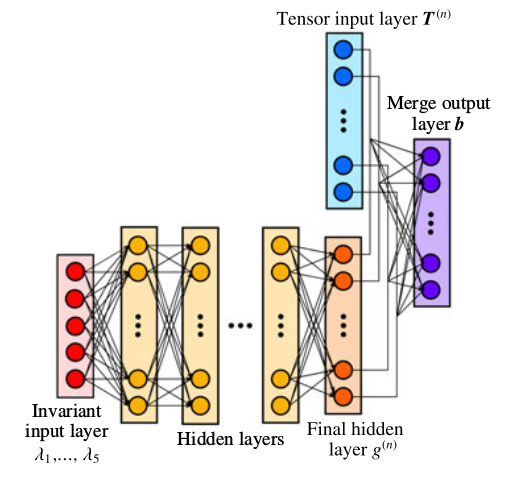
\includegraphics[scale=0.5]{TBNN.png}
\caption{Tensor embedded NN from \citep{kutz2017deep} et \citep{ling2016reynolds}}
\label{TBNN}
\end{figure}
 
\noindent Cette forme de neurones à pour but l'écriture du tenseur anisotropique comme une combinaison linéaire d'une base de tenseur bien particulière.  Les coefficients de cette combinaison sont différentes fonctions des invariants du problème. L'article se base sur les travaux de \cite{pope1975more} et de \cite{smith1965isotropic}.\\
On alors propose de modifier l'hypothèse de Boussinesq qui consistait à écrire 
\begin{equation*}
\bar{u_i' u_j'} = \frac{2}{3} k \delta_{ij} - 2 \nu_t \bar{S_{ij}}
\end{equation*}
 Il propose plutôt de calculer 
\begin{equation*}
\frac{\bar{u_i' u_j'} }{2k}= \frac{1}{3} \delta_{ij} + \sum_\lambda G^\lambda T^\lambda_{ij} 
\end{equation*}
Avec une forme bien particulière pour $G$ et $T$. La première est une fonction des invariants du problème qui sont dans le cas tridimensionnel : 
\begin{equation*}
\mathbf{\Omega}= \left \{ \{\textbf{S}^2\}, \{\textbf{R}^2\}, \{\textbf{S}^3\}, \{\textbf{R}^2\textbf{S}\}, \{\textbf{R}^2 \textbf{S}^2\}\right \} 
\end{equation*}

\noindent La notation $\textbf{\{\}}$ symbolise la trace du tenseur concerné. À noter, que l'invariant $\{\textbf{S}\}$ n'est pas utilisé directement (puisque nul) mais indirectement au travers l'utilisation du $\{\textbf{S}^3\}$. Également, les tenseurs considérés $\textbf{S}$ et $\textbf{R}$ sont définis par 
\begin{align*}
\textbf{S} &= \frac{k}{2\varepsilon}\left(\nabla_x\textbf{U} + \nabla^T_x\textbf{U} \right) \\[0.2cm]
\textbf{R} &= \frac{k}{2 \varepsilon}\left(\nabla_x\textbf{U} - \nabla^T_x\textbf{U} \right) 
\end{align*}

\pagebreak 

\noindent $T$ est composée de 10 tenseurs dans le cas tridimensionnel. Les 10 tenseurs proposés par \cite{pope1975more} et repris par \cite{ling2016reynolds} sont : \setlength{\columnseprule}{0pt}
\\
\vspace{-6mm}
\begin{multicols}{2}

\begin{align*}
\textbf{T}^{(1)} &= \textbf{S} \\
\textbf{T}^{(2)} &= \textbf{S}\textbf{R} - \textbf{R}\textbf{S} \\
\textbf{T}^{(3)} &= \textbf{S}^2 - \dfrac{1}{3}\, \textbf{I} \cdot \text{Tr} \left( \textbf{S}^2 \right)\\
\textbf{T}^{(4)} &= \textbf{R}^2 - \frac{1}{3}\, \textbf{I} \cdot \text{Tr} \left( \textbf{R}^2 \right)\\
\textbf{T}^{(5)} &= \textbf{R}\textbf{S}^2 - \textbf{S}^2\textbf{R}
\end{align*}

\columnbreak

\begin{align*}
\textbf{T}^{(6)} &= \textbf{R}^2\textbf{S} + \textbf{S}^2\textbf{R} - \frac{2}{3}\, \textbf{I}\cdot \text{Tr}\left(\textbf{S}\textbf{R}^2 \right) \\
\textbf{T}^{(7)} &= \textbf{R}\textbf{S}\textbf{R}^2 - \textbf{R}^2\textbf{S}\textbf{R} \\
\textbf{T}^{(8)} &= \textbf{S}\textbf{R}\textbf{S}^2 - \textbf{S}^2\textbf{R}\textbf{S} \\
\textbf{T}^{(9)} &= \textbf{R}^2\textbf{S}^2 + \textbf{S}^2\textbf{R}^2 - \frac{2}{3}\, \textbf{I}\cdot \text{Tr}\left(\textbf{S}^2\textbf{R}^2 \right)\\
\textbf{T}^{(10)} &= \textbf{R}\textbf{S}^2\textbf{R}^2 - \textbf{R}^2\textbf{S}^2\textbf{R}
\end{align*}

\end{multicols}

\noindent Si $T$ peut être calculé en cours de processus, le calcul de $G$ reste encore obscur et justement les coefficients par rapport aux invariants sont définis par le training du NN utilisé ici avec 8 HL \footnote{La dernière HL en aura 10.}, 30 nœuds chacune et $learning\_rate = 2.5 \times 10^{-6}$. \\

Comme on peut le voir Fig.\eqref{TBNN}, les invariants sont injectés en entrée du réseau, suivent ensuite un processus classique propre au Feed-Forward NN. La dernière HL représentera les combinaisons linéaires de coefficients et de la base $\mathbf{\Omega}$. \\
L'output s'écrira alors : $$ b_{ij} = \sum_{n=1}^{10} g^{(n)}(\lambda_1,..,\lambda_5) T_{ij}^{(n)}$$ \\

\noindent Il semblerait que ce réseau soit fait pour déduire l'anisotropie après calcul du modèle RANS. La prédiction à chaque itération fait partie d'un projet qu'ils ont évoqué dans leur article. Les auteurs proposent de comparer les résultats de leurs méthodes avec les DNS de plusieurs cas et avec d'autres méthodes de reconstruction de $\textbf{\textit{b}}$.\\
Le calcul de l'erreur sur l'anisotropie est donné par la formule : 
\begin{equation*}
\text{RMSE} = \sqrt{\frac{1}{6N_{data}} \sum^{N_{data}}_{m=1} \sum^{3}_{i=1} \sum^3_{j=1} \bepar{b_{ij,m,\text{predicted}} - b_{ij,m,\text{DNS}}}^2  }
\end{equation*}
On rapporte les erreurs calculés pour MLP et TBNN dans les cas d'un écoulement en conduite et d'un écoulement au dessus d'une surface présentant une cavité : \\

 \begin{table}[!ht]
\centering
		% Table itself: here we have two columns which are centered and have lines to the left, right and in the middle: |c|c|
		\begin{tabular}{M{.3\textwidth} M{.3\textwidth} M{.3\textwidth} N}
		Modèle & RMSE on Duct Flow & RMSE on Wavy flow &\\[0.15cm]\hline
		\dgreen \textbf{MLP} \bk & 0. 31 & 0.09 &\\[0.2cm]		
		\dpurple \textbf{TBNN} \bk& 0.14 & 0.08 &\\[0.2cm]
		\end{tabular}
		\caption{Comparaisons des erreurs par rapport à la DNS.}
\end{table}

Ils ont également mis en exergue le fait que les erreurs ne provenaient pas seulement de la modélisation du terme anisotrope dans l'hypothèse de Boussinesq; mais également des équations de transports et des différentes approximations mises aux points dans le cadre de l'obtention de ces équations.\\

Un fait soulignable : le training set n'avait de cas semblable à celui du \textit{wavy wall} et malgré tout le TBNN a réussi à fournir une amélioration par rapport aux modèles existants.\\
Ceci prouve que le TBNN est un outil adapté pour la tâche engagée par les auteurs.
\pagebreak

\subsection*{\cite{wu2018data}}
Dans cette article, l'auteur cherche à reconstruire le tenseur d'anisotropie obtenu à partir d'une simulation RANS, à l'aide du Machine learning. On détaille les différentes méthodes et notions mentionnées. On explicitera les différentes régressions et l'expression des différents termes.\\

\noindent En se base sur \cite{pope1975more} , il écrit également le tenseur déviatorique \textbf{b} comme : 
\begin{equation*}
\textbf{b} = \sum_{n=1}^{10} G^{(n)} \mathcal{T}^{(n)}
\end{equation*}
De plus, on lie le Tenseur de Reynolds \textbf{$\tau$} avec $\textbf{b}$ par la relation \begin{equation*}
\mathbf{\tau }= \textbf{b} + \text{Tr}\bepar{\mathbf{\tau}} 
\end{equation*}

\noindent On décompose ensuite le tenseur déviatorique en une partie linéaire et une partie non linéaire :
\begin{equation*}
\textbf{b} = \nu_t^L\textbf{S} + \textbf{b}^\perp
\end{equation*}
Ce qui nous permet de réécrire 
\begin{align*}
\mathbf{\tau }&= \nu_t^L\textbf{S} + \textbf{b}^\perp + \text{Tr}\bepar{\mathbf{\tau}} \\
&= \nu_t^L\textbf{S} + \text{Tr}\bepar{\mathbf{\tau}}  + \textbf{b}^\perp \\
&= \tau^L + \textbf{b}^\perp
\end{align*}

\noindent On exprime à présent $\nu_t^L$, la viscosité turbulente opitmale, en minimisant l'écart entre \textbf{b} et sa partie linéaire : $$\nu_t^L = \underset{\nu_t}{\text{argmin}} \norm{\textbf{b} - \nu_t\textbf{S}} $$
Avec $\norm{\, {•} \, }$ la norme au sens de Frobenius : $\norm{\textbf{S}} = \sqrt{S_{ij}S_{ij}}$. La minimisation précédente revient en fait à calculer $$ \nu_t^L = 2\,  \frac{\textbf{b}:\textbf{S}}{\norm{\textbf{S}} \norm{\textbf{S}}}$$ Où \textbf{b} : \textbf{S} $= b_{ij}S_{ij}$.
On rappelle enfin l'équation dite de \textsc{rans} :
$$ \frac{D\overline{U} }{Dt} + \nabla \overline{P} - \nu \nabla^2 \overline{U} = \nabla \cdot \tau$$
\noindent Toutes les grandeurs ayant été introduites, on construit les features \textbf{q}.\\[2mm]

\subsubsection*{Features \textbf{q}}
\noindent\cite{ling2016reynolds} en suivant \cite{pope1975more} écrivent \textbf{$\tau$} comme une fonctionnelle $\tau\bepar{\textbf{S},\, \mathbf{\Omega}}$ du tenseur de déformations \textbf{S} et du tenseur de rotations \textbf{$\Omega$}, considérant que les effets des gradients de pressions n'agissaient pas sur ce tenseur. \\
De plus, ils ont supposé une turbulence à l'équilibre avec $\mathcal{P} = \mathcal{\varepsilon}$. Dans ce cas, on pourrait simplement écrire $\tau \sim \nabla \overline{U}\bepar{\textbf{x}}$, négligeant ainsi les effets de convection et de diffusion de la turbulence (le non-équilibre de la production et de la dissipation finalement), rendant incomplète la correction cherchée.\\
Il propose une écriture de cette fonctionnelle prenant en compte les grandeurs mentionnées au travers leur gradient :$$\tau = \mathcal{F}\bepar{\textbf{S}, \mathbf{\Omega}, \nabla p, \nabla k}$$ Avec $\mathcal{F}$ une fonction invariante par rotation, pour chacun de ses arguments.\\
L'invariance rotationnelle peut être assurée en choisissant comme entrées la base intègre minimale de l'ensemble $\hat{\mathcal{Q}}  = \beacc{\textbf{S}, \mathbf{\Omega}, \nabla p, \nabla k}$ le chapeau signifiant que les entrées sont adimensionnalisées (on y reviendra), et les invariants de $\tau$ en sortie.\\
La base intègre contient ici 47 éléments listées dans l'annexe B de l'article. L'invariance Galiléenne ne se limitant pas à l'invariance par rotation. Les invariants choisis vérifient l'invariance \textit{Galiléenne} exceptés ceux qui comprennent le $\nabla p$ adimensionnalisés par $\rho \left \vert \overline{U} \cdot \nabla \overline{U} \right \vert$. \\

\noindent Trois autres caractéristiques ont été sélectionnés pour leur sens physique et pour aider la décision de l'IA. Ces trois features sont issus d'un article antérieur \footnote{Les points importants de cet article en question étant similaires à celui là, nous aggrémentons les deux articles} et sont :
\begin{itemize}[leftmargin=3cm]
\item[$q_1$] : indique la distance entre le point en question et le mur. Sert à déterminer si des effets visqueux sont à prendre en compte ou non. $$ q_1 = \text{min}\bepar{\frac{\sqrt{k}\, d}{50 \nu}, 2} \text{, Déjà normalisé }$$
\item[$q_2$] : fournit des informations sur l'échelle spatiale de la turbulence. Cette l'intensité turbulente $k$. On le normalise par $$\frac{1}{2}\, \overline{U_i}\ \overline{U_i}$$
\item[$q_3$] : fournit des informations sur l'échelle temporelle de la turbulence. C'est le rapport de l'échelle spatiale de la turbulence sur l'échelle temporelle moyenne du taux de féformation. $$q_3 = \frac{k}{\varepsilon} \text{, \hspace{5mm} Normalisé par } \, \frac{1}{\norm{\textbf{S}}}$$
\end{itemize}

\subsubsection*{Output du ML}
\pagebreak

\begin{table}[!ht]
		% Center the table
		\centering
		% Table itself: here we have two columns which are centered and have lines to the left, right and in the middle: |c|c|
		\begin{tabular}{|M{.2\textwidth}|M{.74\textwidth}|N }
		\hline
		Auteur & Travaux &\\[.5cm] \hline

		\textbf{\cite{ling2015evaluation}} & Used \red Random Forests (RF) \bk to \navy predict regions of high model from uncertainty in RANS results.\bk &\\[1.5cm] \hline

		\textbf{\cite{ling2016machine}} &Use of \red RF \bk with Gini Impurity Score, max\_depth = 15  and 500 DT whose output are averaged, and \red NN\bk with sigmoid activation function. In the previous work, Ling et \textit{al.} predict the Reynolds Stress Anisotropy $\textbf{A} = \frac{1}{2k} \bar{\textbf{u} \otimes \textbf{u}} - \frac{1}{3}\textbf{Id}$ en un point à partir des images de \textbf{S} et \textbf{R} par les vecteurs d'une base d'invariants bien choisie, en tout point du domaine, ou aux points dont l'incertitude est la plus grande. Les entrées peuvent être aussi bien les invariants de la base que les 9 composantes non nulles cumulées de $\textbf{S}$ et $\textbf{R}$.&\\[4.5cm] \hline		
		
		\textbf{\cite{ling2016reynolds}} & Use of \red NN \bk embbeded with an invariant Tensor Layer element-wise mutliplied with the last HL of the Network. Use of leakyReLu act function. Trained with BPGD, the output is post-processed (see part.2, p.157). It has 8 HL, with each 30 nodes except for the last HL that has 10 nodes and $learning\_rate = 2.5 \times 10^{-7}$. «\textit{Cross Validation ensures robustness of the TBNN}». &\\[3.5cm]\hline		
		
		\textbf{\cite{milano2002neural}} & Used DNS results for a turbulent channel flow to train a \red NN \bk to reconstruct the \navy near wall flow \bk&\\[1.5cm] \hline
		
		\textbf{\cite{tracey2013application}} & ML algorithms (\red??\bk) to model the \navy Reynolds stress anisotopy\bk  &\\[1.5cm] \hline
		
		\textbf{\cite{tracey2015machine}} & \red NN \bk to \navy mimic the source terms from the SA turbulence model \bk &\\[1.5cm] \hline
				
		\textbf{\cite{duraisamy2015new}} & \red NN and GP \bk to \navy model intermittency in transitional turbulence \bk &\\[1.5cm] \hline 		
		
		\textbf{\cite{zhang2015machine}} & Used \red NN and GP \bk to \navy model turbulence Production in channel flow \bk &\\[1.5cm] \hline
		
		\textbf{\cite{singh2017machine}} &Use \red NN \bk to augment SA model to predict turbulent flow over airfoils (strong adverse pressure gradient). First of all use adjoint-based full field inference to infer $\beta$ the correction needed between SA and DNS or Exp. The \red NN \bk proposed here has 2 HL with 100 nodes each, using sigmoid act function. The training used BPGD minimizing an Sum Squarred Error problem.&\\[3cm] \hline 
				
		\end{tabular} 
		\vspace{0.5cm}
		
%		\caption{Tableau retraçant les études NN vs Turbulence faites auparavant 
%		\label{tab:simParameters}}
\end{table}

\pagebreak

\bibliographystyle{apalike}
\bibliography{bibliotheque}

\end{document}